\section{Introduction}
At the end of the PBA stage, we obtain a set of 50-80 keyframes whose camera poses are known with high accuracy, and a coarse face mesh fitted to the landmarks from Openface. Next, we use these keyframes to generate a dense point cloud of the face geometry using Multi-view stereo.


\section{Our Approach}
 We use the parallelized multi-view PatchMatch implementation of Galliani \etal \cite{galliani2015massively} and use 12 source views for each reference view for depth inference. The multi-view PatchMatch estimates a depth map for each of the keyframes. We initialize the depths and search range using the coarse mesh.


To select which source views to use to infer the depth map of a reference view, we calculate a view selection score \cite{yao2018mvsnet} for each pair of keyframes, $s(i, j) = \sum_{\mathbf{p}} \mathcal{G}(\theta_{ij}(\mathbf{p}))$ , where $\mathbf{p}$ is a point common to both views and its baseline angle between the cameras $\mathbf{c}_i$ and $\mathbf{c}_j$ is $\theta_{ij}(\mathbf{p}) = (180/\pi)\arccos((\mathbf{c}_i - \mathbf{p}) \cdot (\mathbf{c}_j - \mathbf{p}))$.  $\mathcal{G}$ is a piecewise Gaussian, as follows :
\[ \mathcal{G}(\theta) =  \left\{
\begin{array}{ll}
      \exp(-\frac{(\theta - \theta_0)^2}{2\sigma_1^2}), \theta \leq \theta_0 \\
      \exp(-\frac{(\theta - \theta_0)^2}{2\sigma_2^2}), \theta > \theta_0 \\
\end{array} 
\right. \]
For our method, we pick $\theta_{0} =10 $  , $\sigma_{1} =5$  and $\sigma_2=10$  .
 We use the estimated coarse mesh to filter out noisy patches in the depth maps produced by the PatchMatch. We then project the depth maps to a single fused point cloud using the fusion strategy proposed in \cite{galliani2015massively}.

Example point clouds output at this step are visualized in Fig \ref{fig:pcl_sample}. 

\begin{figure}[t]
\begin{center}
   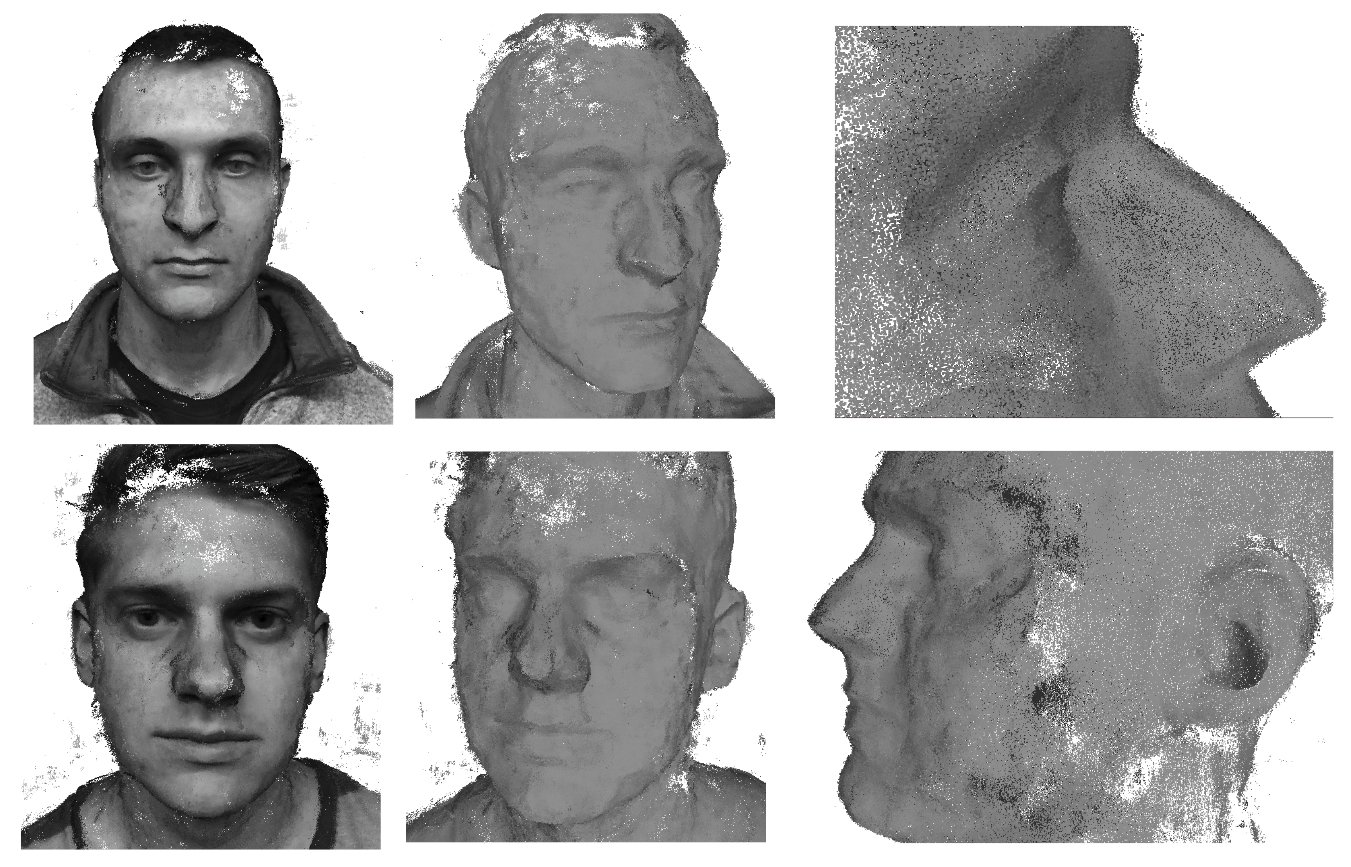
\includegraphics[width=0.95\linewidth]{images/point_clouds_sample.png}
\end{center}
% \vspace{-15pt}
   \caption{Example point clouds generated at the end of our Point cloud generation stage, with and without texture. The point clouds accurately capture the overall face geometry and details in areas like eyes and lips, that make the person recognizable. However, the point clouds have missing data as well as noise, which requires a robust mesh fitting approach (\ref{sec:mesh_fit}).}
\label{fig:pcl_sample}
\end{figure}
